% multilinearalgebra.tex
%
% Copyright (C) 2020-2025 José A. Navarro Ramón <janr.devel@gmail.com>

\chapter{Multilinear algebra}
Multilinear algebra is the same field as linear algebra, it just emphasizes on multilinear maps
instead of only on linear maps. So the object of multilinear algebra is just vector spaces.

Before we continue, let's make it clear from the beginning that
\begin{quotation}
  ``We will not equip physical space (or later, spacetime) with a vector space structure.''
\end{quotation}

You might think we would, because before we had a set and we equipped it with a topological
structure. The point is that we can't do that. Just think about this: if we could equip space with
a vector space structure, then we would know where is $5\cdot \text{Paris}$ or
$\text{Paris} + \text{Vienna}$. But this doesn't make any sense.

However, \emph{tangent spaces}\footnotemark{} ($\text{TpM}$) are objects that can be written as
\emph{smooth manifolds}\footnotemark{} and carry a vector space structure.
\footnotetext{A tangent space is a deceptively intuitive notion that will be explained on
  chapter 5.}
\footnotetext{Smooth manifolds will be seen on chapter 4.}

Very roughly you can think of them (but in fact they will be defined differently) if you think of
the real world as a sphere $M$, then we can associate to every point $p$ in the sphere with
a plane that is tangent to the sphere at this point. In figure~\ref{fig:mla-two-tangent-planes}
the sphere represents the real world (the Earth's surface) and two arbitrary tangent planes TpM
and TqM are drawn on it.
Note that lines on the sphere are there only to highlight perspective. These lines might also be
understood as a certain chart map (longitude and latitude) projected onto the real world,
but this is fantasy, the real world does not care.
\begin{figure}[ht]
  \def\scl{.95}
  % Background
  \pgfmathsetmacro{\BGTOP}{2.6}
  \pgfmathsetmacro{\BGBOTTOM}{-2.2}
  \pgfmathsetmacro{\BGRIGHT}{2.9}
  \pgfmathsetmacro{\BGLEFT}{-2.6}
  %
  \centering
  \begin{tikzpicture}[%
    scale=\scl,
    background/.style={
      line width=\bgborderwidth,
      draw=\bgbordercolor,
      fill=\bgcolor,
    },
    ]
    % Center of sphere
    \coordinate (O) at (3.65,4.2);
    % M, TpM and TqM coordinates
    \coordinate (M) at ($(O) + (-1.7,-1.4)$);
    \coordinate (TpM) at ($(O) + (1.2,2.0)$);
    \coordinate (TqM) at ($(O) + (2.0,-1.2)$);
    % Background coordinates
    \coordinate (bgtop) at ($(O) + (0,\BGTOP)$);
    \coordinate (bgleft) at ($(O) + (\BGLEFT,0)$);
    \coordinate (bgright) at ($(O) + (\BGRIGHT,0)$);
    \coordinate (bgbottom) at ($(O) + (0,\BGBOTTOM)$);
    % PGFPLOTS
    \begin{axis}[%
      colormap name=GY,
      hide axis,
      axis equal,
      width=10cm,
      height=10cm,
      axis lines = center,
      xlabel = {$x$},
      ylabel = {$y$},
      zlabel = {$z$},
      ticks=none,
      enlargelimits=0.3,
      view/az=150,
      scale uniformly strategy=units only,
      ]
      \addplot3[%
      opacity = 1,
      surf,
      z buffer = sort,
      samples = 42,
      variable = \u,
      variable y = \v,
      domain = 0:180,
      y domain = 0:360,
      ]
      % SPHERE u-> phi, v-> theta, r-> 1
      ({cos(u)*sin(v)}, {sin(u)*sin(v)}, {cos(v)});
      
      % ------------------------------------------
      % NORTH POLE P(0,0,1) o r=1, theta=0, phi=0
      % Tangent plane TpM drawing
      \newcommand{\tanPlaneUp}
      {\tanPlaneSph{1}{0}{0}{0}{.5}{.5}}
      \draw[fill=white, fill opacity=.8] \tanPlaneUp -- cycle;
      % Point p r=1  theta=0  phi=0
      \newcommand*{\pointUp}
      {\pointSphPath{1}{0}{0}}
      \filldraw[fill=black,draw=black, ultra thin]
      \pointUp circle[radius=.8pt];
      % Point p label
      \node[anchor=west] at \pointUp {\scriptsize $p$};
      
      % ------------------------------------------
      % ROTATED POINT q: r=1, theta=70, phi=90
      % Rotated tangent plane TqM
      \newcommand{\tanPlaneRot}
      {\tanPlaneSph{1}{70}{90}{0}{.5}{.5}}
      % Tangent plane TqM drawing
      \draw[fill=white, fill opacity=.8] \tanPlaneRot -- cycle;
      % Rotated point q r=1  theta=70  phi=90
      \newcommand*{\pointRot}
      {\pointSphPath{1}{70}{90}}
      \filldraw[fill=black,draw=black, ultra thin]
      \pointRot circle[radius=.8pt];
      % Point q label
      \node[below right=-3pt and 0pt]
      at \pointRot {\scriptsize $q$};
    \end{axis}
    % M, TpM and TqM labels
    \node at (M) {\footnotesize $M$};
    \node at (TpM) {\footnotesize $\text{TpM}$};
    \node at (TqM) {\footnotesize $\text{TqM}$};
    % 
    % YELLOW BACKGROUND 
    % \filldraw[fill=red,draw=black] (bgtop) circle[radius=1pt];
    % \filldraw[fill=red,draw=black] (bgbottom) circle[radius=1pt];
    % \filldraw[fill=green,draw=black] (bgleft) circle[radius=1pt];
    % \filldraw[fill=green,draw=black] (bgright) circle[radius=1pt];
    % \filldraw[fill opacity=0,draw=black] (O) circle[radius=2pt];
    \begin{scope}[on background layer]
      \node [background, fit= (bgleft) (bgright) (bgtop) (bgbottom)] {};
    \end{scope}
  \end{tikzpicture}
  \caption{Two tangent planes TpM and TqM are represented in arbitrary points $p$ and $q$ of the
    real world $M$. Lines on the sphere are drawn only to highlight perspective.}
  \label{fig:mla-two-tangent-planes}
\end{figure}

Tensors, which are very important objects in differential geometry, can be derived from tangent
spaces.

It is beneficial to first study vector spaces and all that comes with it, abstractly, for two
reasons:
\begin{enumerate}
\item For construction of tangent spaces one needs an intermediate vector space denoted as
  $C^\infty (M)$, whatever that will be.
\item Tensor techniques are most easily understood in an abstract setting, without worrying about
  specific examples of $\text{TpM}$ as in figure~\ref{fig:mla-two-tangent-planes}. Tensors can be
  defined in any vector space.
\end{enumerate}


\section{Real vector spaces}
Vector spaces are objects that are studied in linear algebra.

\subsection{Definition}
A real vector space $(V,+_{\scriptscriptstyle V},\cdot_{\scriptscriptstyle V})$ is an algebraic
structure consisting of
\begin{itemize}
\item A set $V$. Most of the time, we will identify $V$ with tangent spaces. But beware that,
  normally, every tangent space is equipped with a different vector space.
\item Addition, which takes two vectors and it maps them to a vector
  \[
    +_{\scriptscriptstyle V} : V\times V \longrightarrow V
  \]
\item S-multiplication\footnotemark{},
  \footnotetext{Stands for scalar multiplication, but we'll never use that word.}
  which takes an real number\footnotemark{} and a vector
  and maps them to a vector
  \[
    \vysmblkcircle_{\scriptscriptstyle V} : \symbb{R}\times V \longrightarrow V
  \]
  \footnotetext{Scalars are real numbers in real vector spaces, and complex numbers in complex
    vector spaces.}
  
  \vspace{-2ex}
  Satisfying these axioms\footnotemark{}:
  \footnotetext{Mnemonics: CANI for addition and ADDU for S-multiplication.}
  
  \def\hspc{.5}
  \begin{description}
  \item[$\text{C}^+$] Commutative property:
    $\forall\vvv{u},\vvv{v}\in V, \hspace{\hspc em}
    \vvv{u} +_{\scriptscriptstyle V} \vvv{v} = \vvv{v} +_{\scriptscriptstyle V} \vvv{u}$.
  \item[$\text{A}^+$] Associative property:
    $\forall \vvv{u},\vvv{v},\vvv{w}\in V, \hspace{\hspc em}
    (\vvv{u} +_{\scriptscriptstyle V} \vvv{v}) +_{\scriptscriptstyle V} \vvv{w}
    = \vvv{u} +_{\scriptscriptstyle V} (\vvv{v} +_{\scriptscriptstyle V} \vvv{w})$.
  \item[$\text{N}^+$] Neutral or identity element:
    $\exists \vvv{0}\in V | \vvv{u} +_{\scriptscriptstyle V} \vvv{0} = \vvv{v},
    \hspace{\hspc em}\forall \vvv{u}\in V$.
  \item[$\text{I}^+$] Inverse elements:
    $\forall \vvv{u}\in V, \exists\vvv{-u}\in V | \vvv{u} +_{\scriptscriptstyle V} (\vvv{-u}) = \vvv{0}$
  \item[$\text{A}^\vysmblkcircle$] Associative property:
    $\forall \lambda, \mu\in\symbb{R}, \forall \vvv{u}\in V, \hspace{\hspc em}
    (\lambda \cdot_{\scriptscriptstyle\symbb{R}} \mu) \cdot_{\scriptscriptstyle V} \vvv{u}
    = \lambda \cdot_{\scriptscriptstyle V} (\mu \cdot_{\scriptscriptstyle V} \vvv{u})$.
  \item[$\text{D}^\vysmblkcircle$] Distributive property
    $\forall \lambda\in\symbb{R}, \forall \vvv{u},\vvv{v}\in V, \hspace{\hspc em}
    \lambda \cdot_{\scriptscriptstyle V} (\vvv{u} +_{\scriptscriptstyle V} \vvv{v})
    = \lambda\cdot_{\scriptscriptstyle V}\vvv{u} +_{\scriptscriptstyle V} \lambda\cdot_{\scriptscriptstyle V}\vvv{v}$
  \item[$\text{D}^\vysmblkcircle$] Distributive property
    $\forall \lambda,\mu\in\symbb{R}, \forall \vvv{u}\in V, \hspace{\hspc em}
    (\lambda +_{\scriptscriptstyle\symbb{R}} \mu) \cdot_{\scriptscriptstyle V} \vvv{u}
    = \lambda\cdot_{\scriptscriptstyle V}\vvv{u} +_{\scriptscriptstyle V} \mu\cdot_{\scriptscriptstyle V}\vvv{u}$    
  \item[$\text{U}^\vysmblkcircle$] Unitary property
    $\exists 1\in\symbb{R} | 1\cdot_{\scriptscriptstyle V}\vvv{u} = \vvv{u},
    \hspace{\hspc em}\forall\vvv{u}\in V$
  \end{description}
  Any structure of this type is a real vector space.
  
  Note: Do not mix up addition and S-multiplication of elements of the vector space,
  $+_{\scriptscriptstyle V}$ and $\cdot_{\scriptscriptstyle V}$ with the same name operations for
  real numbers $+_{\scriptscriptstyle\symbb{R}}$ and $\cdot_{\scriptscriptstyle\symbb{R}}$.
  This distinction is nor really necessary, and can be guessed from the expression.
  But sometimes we'll make it explicit, as in the above definition,  when we want to focus on the
  distinction.
\end{itemize}

Now, a little bit of terminology:
``An element of a vector space is often referred to, informally, as a vector.''

But if someone points at an object and asks whether it is a vector or not, the answer must be than
we don't know. In order to decide, we need to know the $V$, the two operations $+$ and
$\vysmblkcircle$, and check whether the object is an element of $V$ and that the axioms are
satisfied.
This is very important. Even if we have $\symbb{R}^3$, we need to know how to add to triplets
and how to multiply an scalar and a triplet, in order to ask ourselves whether an elmement of
$\symbb{R}^3$ is a vector or not of the vector space $(\symbb{R}^3, +, \vysmblkcircle)$.
Although the component-wise addition of elements of $\symbb{R}^3$ seem natural, there is nothing
natural about it (natural depends on your history). In mathematics you have to specify all that
is required for a concept to be taken into account.

\subsection{Example}\label{subsect:PolynomialExample}
Of course we must know that $(\symbb{R}^n, +, \vysmblkcircle)$, where $n\in\symbb{N}$ are examples
of vector spaces. But following Machiavelli's book ``The Prince'', where he says:
``You have to do the cruel things in the beginning.'', then, instead of writing a single directly
intuitive example\footnotemark{}, we are presenting a more sofisticated one (unless you are a
mathematician) so that it will help us sharpen our understanding of the definitions.
\footnotetext{Because we would probably imagine more than it is written down.}

We define the set $P$ as the set of all maps from the real interval $(-1,+1)$ into the real
numbers, where the maps are of the form $p(x) = \sum_{n=0}^N p_n x^n$
\[
  P\coloneq\Set{p : (-1,+1) \longrightarrow \symbb{R} |
    p(x)= \sum_{n=0}^N p_n x^n, \kern3.pt p_n\in\symbb{R}, \kern3.pt N\in\symbb{N}}
\]
$P$\, is the set of all polynomials of fixed degree $N$.

Now we could ask whether $P$ is a vector space. The short answer is no.
Why? Because $P$\, is a set, and a vector space is a triple $(P,+,\vysmblkcircle)$.
You have to specify also the operations and if they satisfy the axioms, then the triple would be a
vector space.

A similar question would be whether the element $x^2\in P$ is a vector. Short answer again is no.
You have to specify a vector space in the first place\footnotemark{}.
\footnotetext{Often, the vector space is known implicitly and the question may be informally
  acceptable.}

So now we are going to define the operations.
\begin{itemize}
\item Addition of two polynomials:
  \[
    \begin{array}{lccc}
      +_{\scriptscriptstyle P}: & P\times P & \longrightarrow & P\\
         & (p,q) & \mapsto & p +_{\scriptscriptstyle P} q
    \end{array}
  \]
  where
  \[
    (p +_{\scriptscriptstyle P} q) (x) = p(x) +_{\scriptscriptstyle \symbb{R}} q(x)
  \]

  \item S-multiplication of a real number and a polynomial:
  \[
    \begin{array}{lccc}
      \vysmblkcircle_{\scriptscriptstyle P}: & \symbb{R}\times P & \longrightarrow & P\\
         & (\lambda,p) & \mapsto & \lambda \cdot_{\scriptscriptstyle P} p
    \end{array}
  \]
  where
  \[
    (p +_{\scriptscriptstyle P} q) (x) = p(x) +_{\scriptscriptstyle \symbb{R}} q(x)
  \]
\end{itemize}

Let's check the axioms:
\begin{description}
\item[$\text{C}^+$] Commutative property:
  \begin{align*}
    (p + q)(x) &= p(x) + q(x) = \sum_{n=0}^N p_n x^n + \sum_{n=0}^N q_n x^n
                 = \sum_{n=0}^N (p_n + q_n) x^n\\
               &= \sum_{n=0}^N (q_n + p_n) x^n
      = \sum_{n=0}^N q_n x^n + \sum_{n=0}^N p_n x^n = q(x) + p(x)
        = (q + p)(x)
  \end{align*}
\item[$\text{A}^+$] Associative property:
  \begin{align*}
    [(p + q) + r](x)
    &= (p + q)(x) + r(x)
      =(p(x) + q(x)) + r(x)\\
    &= \left(\sum_{n=0}^N p_n x^n + \sum_{n=0}^N q_n x^n\right) + \sum_{n=0}^N r_n x^n\\
    &= \sum_{n=0}^N (p_n + q_n) x^n + \sum_{n=0}^N r_n x^n
      = \sum_{n=0}^N [(p_n + q_n) + r_n] x^n\\
    &= \sum_{n=0}^N [p_n + (q_n + r_n)] x^n
    = \sum_{n=0}^N p_n x^n + \sum_{n=0}^N (q_n + r_n) x^n\\
    &= \sum_{n=0}^N p_n x^n + \left(\sum_{n=0}^N q_n x^n + \sum_{n=0}^N r_n x^n\right)
      = p(x) + (q(x) + r(x))\\
    &= p(x) + (q + r)(x)
    = [p + (q + r)](x)
  \end{align*}
\item[$\text{N}^+$] Identity element:
  
  Consider $o(x) = \sum_{n=0}^N o_n x^n = \sum_{n=0}^N 0\, x^n = 0$, where all the $o_n$ are zero
  \[
    (o + p)(x) = o(x) + p(x) = \sum_{n=0}^N o_n x^n + \sum_{n=0}^N p_n x^n
    = 0 + \sum_{n=0}^N p_n x^n = p(x)
  \]
\item[$\text{I}^+$] Inverse element:
  
  Given a polynomial $p(x) = \sum_{n=0}^N p_n x^n$, we can find another one
  \[
    (-p)(x) = -\sum_{n=0}^N p_n x^n = \sum_{n=0}^N (-p_n) x^n
  \]
  such that
  \begin{align*}
    [p + (-p)](x) &= p(x) + (-p(x)) = \sum_{n=0}^N p_n x^n + \sum_{n=0}^N (-p_n) x^n
               = \sum_{n=0}^N (p_n + (-p_n)) x^n\\
             &=\sum_{n=0}^N 0 x^n = 0 = o(x)
  \end{align*}
\end{description}
Now we leave as an exercise to prove the rest of the axioms.


\section{Linear maps}
It is a standard procedure in mathematics, once you have an object defined, a structure,
a space with a certain structure, that we investigate the structure by considering maps between
one such structure and another instance of such structure.

We did this in topology. We had two topological spaces and we studied maps between them which
respected the structure. In topology it was the open set structure (preimages of open sets are
open). Here we are going to do a similar thing. These are the structure respecting maps between
vector spaces, which are called linear maps or linear transformations.

\subsection{Definition}
A linear map is a homomorphism of vector spaces.
If $(V,+_v,\vysmblkcircle_v)$ and $(W,+_w,\vysmblkcircle_w)$ are two vector spaces, then a map
\[
  \varphi: V \longrightarrow W
\]
is called linear if the following two conditions are satisfied
\begin{enumerate}
\item $\forall v,\tilde v\in V$,\hspace{.5em}
  $\varphi(v +_v \tilde v) = \varphi(v) +_w \varphi(\tilde v)$
\item $\forall\lambda\in\symbb{R}$, $\forall v\in V$,\hspace{.5em}
  $\varphi(\lambda\vysmblkcircle_v v) = \lambda\vysmblkcircle_w \varphi(v)$
\end{enumerate}
All four operations appear on the definition of a linear map. So a linear map connects the two
spaces somehow. Only very special maps will have this property.

As with continuity, which was a nonsensical concept until we know the topology.
Now this is similar. It does not make sense whether a map is linear or not, until you tell me
the complete vector space structure on these sets, the domain and the target.

\subsection{Example}
This example will use the vector space structure of the set of polynomials that we saw before, in
subsection~\ref{subsect:PolynomialExample}.
Let's consider the transformation that maps a polynomial into its derivative, which is another
polynomial
\[
  \begin{array}{lccc}
    \delta : & P & \longrightarrow & P\\
             & p & \mapsto & p'
  \end{array}
\]
The $\delta$ map can be described as a differenciation operator.

Let's check whether this map is linear
\begin{enumerate}
\item First condition
  \[
    \delta(p +_{\scriptscriptstyle P} q)
    = (p +_{\scriptscriptstyle P} q)'
    = p' +_{\scriptscriptstyle P} q'
    = \delta(p) + \delta(q)
  \]
  where we have taken into account that the derivative of a sum of polynomials is
  the sum of their derivatives.
\item Second condition
  \[
    \delta(\lambda \cdot_{\scriptscriptstyle P} p)
    = (\lambda \cdot_{\scriptscriptstyle P} p)'
    = \lambda \cdot_{\scriptscriptstyle P} p'
    = \lambda \cdot_{\scriptscriptstyle P} \delta(p)
  \]
  whre we have taken into account that the derivative of a constant times a polynomial
  is the constant times the derivative of the polynomial.
\end{enumerate}
So the differential operator $\delta$ acting on polynomials is a linear map.

\subsubsection{Notation}
In order to save a lot of writing, we can avoid saying that some map $\varphi$ is linear,
by writing a tilde above or below the arrow, like that
\vspace{-1ex}
\begin{center}
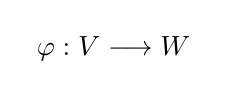
\begin{tikzpicture}
  \node[label={[xshift=.9em,yshift=-1.75ex]{\footnotesize $\invlazys$}}] {$\varphi : V \longrightarrow W$};
\end{tikzpicture}
\end{center}

% \mappic{$\varphi : V$}{-.5em}{$\varphi$}{$\invlazys$}{-.5em}{$W$}


\subsection{Linear maps composition}
Let's have two linear maps $\varphi$ and $\psi$
\begin{center}
\begin{tikzpicture}
  \node[label={[xshift=.9em,yshift=-1.75ex,name=phi]
    {\footnotesize $\invlazys$}}] {$\varphi : U \longrightarrow V$};
    \node[below left=2ex and -3.1em of phi,label={[xshift=.8em,yshift=-1.75ex,name=psi]
    {\footnotesize $\invlazys$}}] {$\psi : V \longrightarrow W$};
\end{tikzpicture}
\end{center}

Now we are interested in the composition $\psi\circ\varphi$ of these two linear maps
\begin{center}
  \begin{tikzpicture}
    % U
    \node[name=U] {$U$};
    % arrow 1
    \node[name=arrow1,right=-.2em of U] {$\longrightarrow$};
    \node[above] at (arrow1) {\footnotesize $\varphi$};
    \node[below] at (arrow1) {\footnotesize $\invlazys$};
    % V
    \node[name=V,right=-.35em of arrow1] {$V$};
    % arrow 2
    \node[name=arrow2,right=-.2em of V] {$\longrightarrow$};
    \node[above] at (arrow2) {\footnotesize $\psi$};
    \node[below] at (arrow2) {\footnotesize $\invlazys$};
    % W
    \node[name=W,right=-.35em of arrow2] {$W$};
    % Map composition
    \draw[-{Latex[round]}] (U) to[out=280,in=260] node[below] {\footnotesize $\psi\circ\varphi$} (W);
\end{tikzpicture}
\end{center}

We claim that \emph{the composition of linear maps is linear}.
To prove this, we need to check that the two conditions for linear maps are satisfied:
\begin{enumerate}
\item The image of the sum is the sum of the images:
  \begin{align*}
    (\psi\circ\varphi) (u_1 + u_2) &= \psi[\varphi(u_1 + u_2)]
                                     = \psi[\varphi(u_1) + \varphi(u_2)]
                                     = \psi[\varphi(u_1)] + \psi[\varphi(u_2)]\\
                                   &= (\psi\circ\varphi) (u_1) + (\psi\circ\varphi) (u_2)
  \end{align*}
  for all $u_1, u_2\in U$.
\item The image of a scalar times a vector is the scalar times the image of the vector
  \begin{align*}
    (\psi\circ\varphi) (\lambda u) &= \psi[\varphi(\lambda u)]
                                     = \psi[\lambda \varphi(u)]
                                     = \lambda \psi[\varphi(u)]
                                   = \lambda (\psi\circ\varphi) (u)
  \end{align*}
  for all $\lambda\in\symbb{R}$ and $u\in U$.
\end{enumerate}

This theorem could also be proved using the concept of basis of a vector space, which will be
introduced at the very end of this chapter. This is because that in order to understand what's
going on you must not introduce a basis. The concept of a basis clouds our thinking. Later on,
using the basis vectors, the composition $\psi\circ\varphi$ will essentially explain the matrix
multiplication rule.

\subsection{Vector space of homomorphisms}
\subsubsection{Definition}
The vector space of homomorphisms is a triple which consists of: 
\begin{enumerate}
\item A set, with the funny name $\text{Hom}(V,W)$.
  Let $(V,+,\vysmblkcircle)$ and $(W,+,\vysmblkcircle)$
  be two real\footnotemark{} vector spaces. Then we can define the set of all linear maps from one
  to the other:
  \footnotetext{Here we consider \emph{real vector spaces}, but this may be applied to any field,
    $\symbb{R}, \symbb{C}, \text{etc.}$}
  \begin{center}
    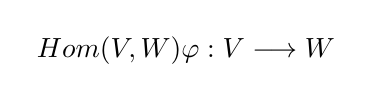
\begin{tikzpicture}
      \node[label={[xshift=4.0em,yshift=-2.0ex] \footnotesize $\invlazys$}]
      {$\text{Hom}(V,W) \coloneq \set{\varphi : V \longrightarrow W}$};
    \end{tikzpicture}
  \end{center}  
  
\item The sum of two linear maps, $+$:
  \[
    \begin{array}{cccc}
      + : & \text{Hom}(V,W) \times \text{Hom}(V,W) &\longrightarrow & \text{Hom}(V,W)\\
               &    (\varphi,\psi)  & \mapsto & \varphi + \psi
    \end{array}
  \]
  where the addition is defined as
  \[
    (\varphi + \varphi)(v) \coloneq \varphi(v) + \varphi(v)
  \]
  
  We define the $+$ on $\text{Hom}(V,W)$ by using the $+$ in $W$.
  Note that we have three additions, $+_{\scriptscriptstyle V}$\,,
  $+_{\scriptscriptstyle W}$ and $+_{\scriptscriptstyle HVW}$, although we won't usually make any
  written distiction between them.

\item The S-multiplication of a scalar times a linear map, $\scriptstyle\odot$:
  \[
    \begin{array}{cccc}
      \vysmblkcircle : & \text{Hom}(V,W) \times \text{Hom}(V,W) &\longrightarrow & \text{Hom}(V,W)\\
               &    (\varphi,\psi)  & \mapsto & \varphi \cdot \psi
    \end{array}
  \]
  which is defined as
  \[
    (\varphi \cdot \varphi)(v) \coloneq \varphi(v) \cdot \varphi(v)
  \]
  
  Note that we have three different S-multiplications,
  $\vysmblkcircle_{\scriptscriptstyle V}$, $\vysmblkcircle_{\scriptscriptstyle W}$ and
  $\vysmblkcircle_{\scriptscriptstyle HVW}$\,.
\end{enumerate}

\subsubsection{Vector space proof}
It is easy to prove that $(\text{Hom}(V,W), +, \vysmblkcircle)$ is a vector space,
given that $(V,+,\vysmblkcircle)$ and $(W,+,\vysmblkcircle)$ are vector spaces.
Let's check the axioms:
\begin{description}
\item[$\text{C}^+$] Commutative property, $\forall \varphi,\psi\in\text{Hom}(V,W)$,\,
  $\varphi + \psi = \psi + \varphi$:
  \[
    \forall v\in V,\,
    (\varphi + \psi)(v) = \varphi(v) + \psi(v) = \psi(v) + \varphi(v) = (\psi + \varphi)(v)
  \]
  %$\forall v\in V$.
\item[$\text{A}^+$] Associative property, $\forall \varphi,\psi,\eta\in\text{Hom}(V,W)$,\,
  $(\varphi + \psi) + \eta = \varphi + (\psi + \eta)$:
  \begin{align*}
    \forall v\in V,\, 
    [(\varphi + \psi) + \eta](v)
    &= (\varphi + \psi)(v) + \eta(v)
      = (\varphi(v) + \psi(v)) + \eta(v)\\
    &= \varphi(v) + (\psi(v)) + \eta(v))
      =\varphi(v) + (\psi + \eta)(v)\\
    &= [\varphi + (\psi + \eta)](v)
      = [\varphi + (\psi + \eta)](v)
  \end{align*}
\item[$\text{N}^+$] Identity element,
  $\exists\,\omicron\in\text{Hom}(V,W)\, |\, \forall\varphi\in\text{Hom}(V,W),\,\omicron + \varphi = \varphi$:\\
  Let $v\in V$, and $\omicron(v) = 0_{\scriptscriptstyle W} = 0\in W$
  be the identity element in $W$
  \[
    (\omicron + \varphi)(v) = \omicron(v) + \varphi(v) = 0 + \varphi(v) = \varphi(v)
  \]
\item[$\text{I}^+$] Inverse element, $\forall\varphi\in\text{Hom}(V,W), \,\exists (-\varphi)\in\text{Hom}(V,W)
  \,|\, \varphi + (-\varphi) = \omicron$:
  \[
    \forall v\in V,\,[\varphi + (-\varphi)](v) = \varphi(v) + (-\varphi(v)) = 0_W = 0 = \omicron(v)
  \]
\item[$\text{A}^\vysmblkcircle$] Associative property,
  $\forall\lambda,\mu\in\symbb{R}, \forall\varphi\in\text{Hom}(V,W), \,(\lambda\cdot\mu) \cdot \varphi
  = \lambda\cdot(\mu\cdot \varphi)$
  \[
    [(\lambda\cdot\mu)\cdot \varphi](v)
    = (\lambda\cdot\mu) \cdot \varphi(v) = \lambda \cdot (\mu \cdot\varphi(v))
    = \lambda \cdot (\mu\cdot\varphi)(v)
    = [\lambda\cdot(\mu\cdot\varphi)](v)
  \]
\item[$\text{D}^\vysmblkcircle$] Distributive property,
  $\forall\lambda,\mu\in\symbb{R}, \forall\varphi\in\text{Hom}(V,W), \,
  \lambda\cdot(\varphi + \psi) = \lambda\cdot\varphi + \lambda\cdot\psi$
  \begin{align*}
    [\lambda\cdot(\varphi + \psi)](v)
    &= \lambda\cdot (\varphi + \psi)(v)
      = \lambda\cdot (\varphi(v) + \psi(v))
      = \lambda\cdot\varphi(v) + \lambda\cdot\psi(v)\\
    &= (\lambda\cdot\varphi)(v) + (\lambda\cdot\psi)(v)
      = [\lambda\cdot\varphi + \lambda\cdot\psi](v)
  \end{align*}
\item[$\text{D}^\vysmblkcircle$] Distributive property,
  $\forall\lambda,\mu\in\symbb{R}, \forall\varphi\in\text{Hom}(V,W), \,
  (\lambda+\mu)\cdot\varphi = \lambda\cdot\varphi + \mu\cdot\varphi$
  \begin{align*}
    \forall v\in V,\,
    [(\lambda + \mu) \cdot\varphi](v)
    &= (\lambda + \mu) \cdot \varphi(v)
      = \lambda\cdot \varphi(v) + \mu\cdot\varphi(v)
  \end{align*}
\item[$\text{U}^\vysmblkcircle$] Unitary property, $1\cdot\varphi = \varphi$
  \begin{align*}
    [1\cdot\varphi](v)
    &= 1\cdot \varphi(v)
      = \varphi(v)
  \end{align*}

\end{description}

So if we start with two vector spaces, you can construct a third one by considering the set
of all the linear maps between the first into the second one, and two the two operations
specified before $(\text{Hom}(V,W),+,\vysmblkcircle)$.

This could be a curiosity, but if we go on and build a new vector space by considering the set of
all linear maps from another pair of vector spaces $\text{Hom}(U,S)$, we could consider the set of
all linear maps
\begin{center}
  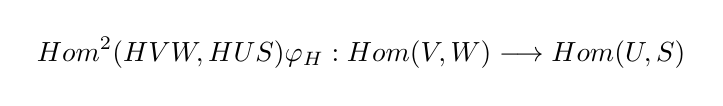
\begin{tikzpicture}
    \node[label={[xshift=6.5em,yshift=-2.4ex] \footnotesize $\invlazys$}]
    {$\text{Hom}^2(HVW,HUS) \coloneq \set{\varphi_H : \text{Hom}(V,W) \longrightarrow \text{Hom}(U,S)}$};
  \end{tikzpicture}
\end{center}
and this way we could get a tower of vector spaces.
We will come back later with this when discussing tensors.

\subsubsection{Example}
Consider $\text{Hom}(P,P)$, where $P$ is our polynomial example, which we used to build a vector
space structure by defining two operations $(P,+,\vysmblkcircle)$. What does it mean?
It means that we can take an element as the derivative operator $\delta\in\text{Hom}(P,P)$, which
is a linear map. But we found that the composition of two linear maps is a new linear map, so
we can form a series of linear maps
\begin{center}
\begin{tabular}{l}
  $\delta\circ\delta\in\text{Hom}(P,P)$\\
  $\delta\circ\delta\circ\delta\in\text{Hom}(P,P)$\\
  \multicolumn{1}{c}{$\cdots$}\\
  $\delta\circ \cdots \circ\delta\in\text{Hom}(P,P)$
\end{tabular}
\end{center}
But, because $\text{Hom}(P,P)$ carries a vector space structure, you can now write things like
\emph{five times the first derivative plus the second derivative}, for instance
\[
  5\circ \delta + \delta\circ\delta \in\text{Hom}(P,P)
\]
and this is something we do all the time when considering the derivatives of a polynomial.
So it is an extremely natural object that we use frequently.


\subsection{Dual vector space}
This is a much scaring topic for students but it is totally unclear why it is so feared.
In fact we already considered it. It is just a heavily used special case.

If we have a vector space $(V,+,\vysmblkcircle)$, then we can define a set $V^\ast$ as all the
linear maps from $V$ into the real numbers, $\symbb{R}$, with the usual addition and multiplication
we learned from basic calculus, which form a vector space, $(\symbb{R},+,\cdot)$
\begin{center}
  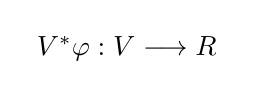
\begin{tikzpicture}
    \node[label={[xshift=2.2em,yshift=-2.0ex]
      {\footnotesize $\invlazys$}}]
    {$V^\ast\coloneq\set{\varphi : V \longrightarrow \symbb{R}}$};
\end{tikzpicture}
\end{center}
The dual space $V^\ast$ is just a special case of $\text{Hom}(V,W)$ which we saw before
\[
  V^\ast = \text{Hom}(V,\symbb{R})
\]
Dual vectors are heavily used. If you know the $V$ and the $V^\ast$, you can construct all the rest.
The triple $(V^\ast,+,\vysmblkcircle)$ is a vector space, and it is called the
\emph{dual vector space (to $V$)}.
Note that the dual vector space $V^\ast$ is just a particular set of linear maps. This should not be
so scary!

\subsubsection{Terminology}
An element $\varphi\in V^\ast$ is called informally a \emph{covector}.
Actually, it is bad terminology because we can call it a \emph{vector}, though it is commonly
accepted to call vectors to elements of $V$ and covectors to elements of the dual vector space
$V^\ast$.

\subsubsection{Example}
Consider a linear map $I$, that goes from $P$ \,into the real numbers. So it must be an element
of the dual space, $I\in P^\ast$
\begin{center}
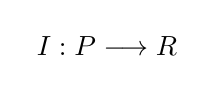
\begin{tikzpicture}
  \node[label={[xshift=.8em,yshift=-1.75ex]{\footnotesize $\invlazys$}}]
  {$I : P \longrightarrow \symbb{R}$};
\end{tikzpicture}
\end{center}

Let's define this specific element $I$ as a map which takes a polynomial and produces
a real number
\[
  I(p) \coloneq \int_0^1 dx\, p(x)
\]

$I$ is a linear map because it satisfies the two conditions:
\begin{align*}
  I(p+q) &= \int_0^1 dx\, (p(x) + q(x)) = \int_0^1 dx\, p(x) + \int_0^1 dx\, q(x) = I(p) + I(q)\\
  I(\lambda\cdot p) &= \int_0^1 dx\, \lambda p(x) = \lambda \int_0^1 dx\,p(x) = \lambda I(p)
\end{align*}
So the definite integration operator, $I=\int_0^1 dx\in P^\ast$, which \emph{eats} a polynomial and
produces a real number is a \emph{covector}.

This is something we use all the time. It is very common in quantum mechanics.
The gradient of a function on $\symbb{R}^n$ is also a covector.
We meet lots and lots of objects in our life as physicists that are covectors, but we started
to learned them as vectors in order not to bother us with these details. In fact, the impression
that \emph{covectors} are something extremely unnatural and something very esoteric is simply
because people have lied to you. They are all around and we have used many examples without
knowing. Of course we will come back with some of these points at a later time.

\subsection{Tensors}
From any vector space you can get a dual space. These are the elementary building blocks to build
the entire tower of vector space structures that we talked before (the entire heap of maps of maps
of maps, etc., between vector space structures).
The elements of these higher and higher structures are generically called \emph{tensors}.
Tensors are such natural objects in Linear Algebra. They apply to all vector spaces and
any vector space dimension\footnotemark{}.
\footnotetext{At the end of the chapter we will introduce the \emph{dimension} and \emph{basis} of
  a vector space. They are useful concepts, but introduce a great deal of arbitrariness in the
  choice of a basis.}

On finite dimensional vector spaces there is a very simple way to think of tensors as multilinear
maps. So we will start with these finite dimensional vector spaces because tangent maps on our
manifolds will be finite dimensional.
The topological manifold dimension $d$ as we defined before, and the tangent vector space dimension
$d$ are different notions of dimension, but the two numbers agree.

\subsubsection{Definition}
Let $(V,+,\vysmblkcircle)$ be a vector space. An (r,s)-tensor $T$ over $V$ is a multilinear map
that \emph{eats} a tuple with the first $r$ copies of $V^\ast$ (covectors) and the next $s$ copies of
$V$ (vectors) to produce a real number
\begin{center}
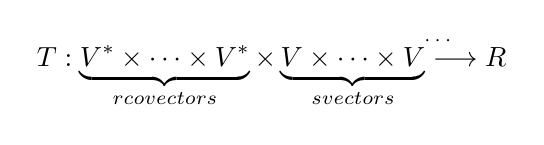
\begin{tikzpicture}
  \node[name=arrow]
  {$T : \underbrace{V^\ast\times\cdots\times V^\ast}_{r\text{ covectors}}
    \times \underbrace{V\times\cdots\times V}_{s\text{ vectors}} \longrightarrow \symbb{R}$};
  \node[label={[xshift=6.0em,yshift=.3ex]{\footnotesize $\invlazys$}}] at (arrow) {};
  \node[label={[xshift=6.0em,yshift=.94ex]{\scriptsize $\cdots$}}] at (arrow) {};
  \node[label={[xshift=6.0em,yshift=1.5ex]{\footnotesize $\invlazys$}}] at (arrow) {};
\end{tikzpicture}
\end{center}
where $r$ and $s$ are non-negative integers: $r,s\in\symbb{N}_0$. The multiple $\invlazys$'s
above the map arrow are there to indicate that the tensor $T$ is multilinear.
On the next examples we are going to maintain this notation, but for simplicity,  in future
examples we will use only one $\invlazys$ to indicate multilinearity.

\subsubsection{Generic example}
Let's consider a generic (1,1)-tensor, $T$, which takes a pair of objects, the first being a
covector and the next one a vector and produces a real number, $T(\varphi, v)\in\symbb{R}$
\begin{center}
\begin{tikzpicture}
  \node[name=arrow]
  {$T : V^\ast \times V \longrightarrow \symbb{R}$};
  \node[label={[xshift=2.0em,yshift=-1.5ex]{\footnotesize $\invlazys$}}] at (arrow) {};
  \node[label={[xshift=2.0em,yshift=-.7ex]{\footnotesize $\invlazys$}}] at (arrow) {};
  \node[below right=1ex and -1.5em] at (arrow)
  {\small $(\varphi,v)\hspace{.6em} \mapsto\hspace{.4em}T(\varphi,v)$};
\end{tikzpicture}
\end{center}
This tensor is multilinear, so it must be linear in the first entry
\[
  \left\{
    \begin{array}{ll}
      T(\varphi + \psi,v) = T(\varphi,v) + T(\psi,v)\\
      T(\lambda\cdot\varphi,v) = \lambda\cdot T(\varphi,v)
    \end{array}
    \right.
\]
and in the second entry
\[
  \left\{
    \begin{array}{ll}
      T(\varphi,v + w) = T(\varphi,v) + T(\varphi,w)\\
      T(\varphi,\lambda\cdot v) = \lambda\cdot T(\varphi,v)
    \end{array}
    \right.
\]

For example, the $T(\varphi + \psi, v + w)$ expression would be expanded as
\[
  T(\varphi + \psi, v + w)
  = T(\varphi,v) + T(\varphi,w) + T(\psi,v) + T(\psi,w)
\]
where we used linearity twice.

\subsubsection{Interesting remark}
Given a map $T$
\begin{center}
\begin{tikzpicture}
  \node[name=arrow]
  {$T : V^\ast \times V \longrightarrow \symbb{R}$};
  \node[label={[xshift=2.0em,yshift=-1.5ex]{\footnotesize $\invlazys$}}] at (arrow) {};
  \node[label={[xshift=2.0em,yshift=-.7ex]{\footnotesize $\invlazys$}}] at (arrow) {};
  \node[below right=.8ex and -1.8em] at (arrow)
  {\small $(\varphi,v)\hspace{.85em} \mapsto\hspace{.5em}T(\varphi,v)$};
\end{tikzpicture}
\end{center}
I define a map $\phi_T$ constructed from the $T$
\begin{center}
\begin{tikzpicture}
  \node[name=arrow]
  {$\phi_T : V \longrightarrow (V^\ast)^\ast$};
  \node[label={[xshift=.15em,yshift=-1.15ex]{\footnotesize $\invlazys$}}] at (arrow) {};
  \node[below right=.8ex and -1.8em] at (arrow)
  {\small $v\hspace{.8em} \mapsto\hspace{.45em}T(\textcolor{gray}{\mdsmwhtsquare},v)$};
\end{tikzpicture}
\end{center}
where we feed the $T$ with the vector but leave the covector slot empty (represented by an empty
square).

But what does $T(\textcolor{gray}{\mdsmwhtsquare},v)$ mean?
This is an hungry object that can eat a covector and produce a real number, according to the
definition of the map $T$. So we could write $T(\textcolor{gray}{\mdsmwhtsquare},v)$ as a map that
\emph{eats} a covector and spits out a real number in linear fashion
\begin{center}
\begin{tikzpicture}
  \node[name=arrow]
  {$T(\textcolor{gray}{\mdsmwhtsquare},v) : V^\ast \longrightarrow \symbb{R}$};
  \node[label={[xshift=2.15em,yshift=-1.15ex]{\footnotesize $\invlazys$}}] at (arrow) {};
  \node[below right=.8ex and -.3em] at (arrow)
  {\small $\varphi\hspace{1.0em} \mapsto\hspace{.5em}r$};
\end{tikzpicture}
\end{center}

Why $\phi_T$ is a map from $V$ into $(V^\ast)^\ast$?
Think that $T(\mdsmwhtsquare,v)$ eats a covector and spits out a real number, but a covector
in nothing more than a vector. So $T(\mdsmwhtsquare,v)$, as a linear map from $V^\ast$ into
$\symbb{R}$ is an element of the dual vector space of $V^\ast$, that is $(V^\ast)^\ast$.

It is a fact that we are not going to prove right here that if $V$ is finite dimensional
$\text{dim} V < \infty$, then $(V^\ast)^\ast = V$. The $V$ star-star reproduces the $V$, but only
for finite dimensional vector spaces.

So we can think of $\phi_T$ as a map from $V$ to $V$
\begin{center}
\begin{tikzpicture}
  \node[name=arrow]
  {$\phi_T : V \longrightarrow V$};
  \node[label={[xshift=1.15em,yshift=-1.15ex]{\footnotesize $\invlazys$}}] at (arrow) {};
  \node[below right=.8ex and -.9em] at (arrow)
  {\small $v\hspace{.8em} \mapsto\hspace{.45em}T(\textcolor{gray}{\mdsmwhtsquare},v)$};
\end{tikzpicture}
\end{center}
and this is the way we like to think as a (1,1)-tensor.

We could have done it the other way round. Start with a linear map which \emph{eats} a vector and
\emph{spits out} a vector
\begin{center}
\begin{tikzpicture}
  \node[name=arrow]
  {$\phi : V \longrightarrow V$};
  \node[label={[xshift=.9em,yshift=-1.15ex]{\footnotesize $\invlazys$}}] at (arrow) {};
  \node[below right=.8ex and -1.2em] at (arrow)
  {\small $v\hspace{.8em} \mapsto\hspace{.45em}u$};
\end{tikzpicture}
\end{center}
and prove that $T_\phi$, constructed from the $\phi$ contains the same data as the $\phi$,
so that they are equivalent
\begin{center}
\begin{tikzpicture}
  \node[name=arrow]
  {$T_\phi : V^\ast \times V \longrightarrow \symbb{R}$};
  \node[label={[xshift=2.2em,yshift=-1.2ex]{\footnotesize $\invlazys$}}] at (arrow) {};
  \node[label={[xshift=2.2em,yshift=-.4ex]{\footnotesize $\invlazys$}}] at (arrow) {};
  \node[below right=.8ex and -1.6em] at (arrow)
  {\small $(\varphi,v)\hspace{.9em} \mapsto\hspace{.5em}\varphi(\phi(v))$};
\end{tikzpicture}
\end{center}

So a linear map from $V$ into $V$ has the same data as a map from $V^\ast\times V$ into $\symbb{R}$,
so $T$ and $\phi_T$ are equivalent, we can think of a (1,1)-tensor as multilinear map
that takes a covector and a vector and produces a real number, or as a linear map that
takes a vector and produces a vector. The two things are the same when the vector space
dimension is finite.

% 1:03:00

\subsubsection{Example}
Let's see an example of a tensor $g$ taking two polynomials and mapping them multilinearly into
the real numbers. The specific map we choose in this example is the some definite integral of the
product of the two polynomials
\begin{center}
\begin{tikzpicture}
  \node[name=arrow]
  {$g : P \times P \longrightarrow \symbb{R}$};
  \node[label={[xshift=1.68em,yshift=-1.2ex]{\footnotesize $\invlazys$}}] at (arrow) {};
  \node[label={[xshift=1.68em,yshift=-.4ex]{\footnotesize $\invlazys$}}] at (arrow) {};
  \node[below right=.8ex and -1.9em] at (arrow)
  {\small $(p,q)\hspace{.87em} \mapsto\hspace{.5em}\int_{-1}^1 dx\,p(x)\kern.8pt q(x)$};
\end{tikzpicture}
\end{center}
This (0,2)-tensor over $P$ is the inner product of two polynomials.

\subsection{Vectors and covectors as tensors}
It is obvious that covectors are vectors, but it is less obvious that vectors are tensors.

A covector $\varphi$ is an element of the dual vector space, $\varphi\in V^\ast$. This is the same as
saying that $\varphi$ is a linear map from $V$ to the real numbers, but that, by definition of
tensors, is a (0,1)-tensor
\begin{center}
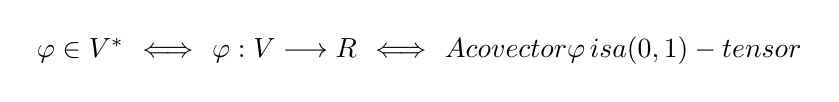
\begin{tikzpicture}
  \node[name=arrow]
  {$\varphi\in V^\ast
    \hspace{.4em}\Longleftrightarrow\hspace{.4em}
    \varphi : V \longrightarrow \symbb{R}
    \hspace{.4em}\Longleftrightarrow\hspace{.4em}
    \text{A covector }\varphi\,\text{ is a (0,1)-tensor}$};
  \node[label={[xshift=-1.28em,yshift=-1.15ex]{\footnotesize $\invlazys$}}] at (arrow) {};
\end{tikzpicture}
\end{center}

A vector space $V$ is the same as $(V^\ast)^\ast$ for a finite dimensional vector space\footnotemark{}
A vector $v\in V = (V^\ast)^\ast$, by definition is the same that $V$ is a linear map from $V^\ast$ into
the real numbers
\footnotetext{Although we didn't proved it.}
\begin{center}
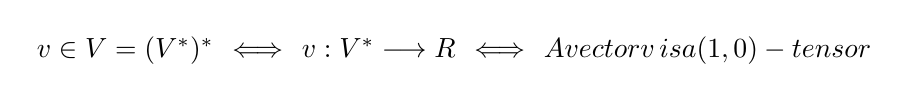
\begin{tikzpicture}
  \node[name=arrow]
  {$v\in V = (V^\ast)^\ast
    \hspace{.4em}\Longleftrightarrow\hspace{.4em}
    v : V^\ast \longrightarrow \symbb{R}
    \hspace{.4em}\Longleftrightarrow\hspace{.4em}
    \text{A vector } v\, \text{ is a (1,0)-tensor}$};
  \node[label={[xshift=-1.4em,yshift=-1.15ex]{\footnotesize $\invlazys$}}] at (arrow) {};
\end{tikzpicture}
\end{center}

Vectors are (1,0)-tensors, covectors are (0,1)-tensors,
inner products on a vector space (if you give one) are (0,2)-tensors. The inverse of an
inner product (the inner product on the dual space) is a (2,0)-tensor, and so on.

So there are many different tensor objects, as the moment of inertia, that we have used in classes
that we had never called them tensors before.

% 1:10:05

\subsection{Basis of a vector space}
So far we have not used the concept of \emph{basis of a vector space}. We do not need this concept
in order to understand vectors and tensors. An introduction to vector spaces should be first
learned without the basis and component notions. We must understand vectors as not being a
collection of numbers, because vectors are just that, they don't have collection of numbers.
If you don't see vectors as collections of numbers you are doing well.

For example, if I write down the polynomial $x^3 - 2x\in P$, I could ask you what is the collection
of numbers of this vector? There's no such collection of numbers in the polynomial.
Of course we could build one, but it is not unique. It depends on other considerations which are
not intrinsic to the nature of vectors. In fact, there are uncountable many ways to assign a such a
collection to vectors. The choice of one of these ways is called a \emph{choice of basis}.

In quantum mechanics the inner product is defined as a (0,2)-tensor of on complex functions.
But if we choose a \emph{basis}, we could calculate the inner product through the vector
components.
If you have uncountable many choices and you pick one of them, you are dealing with a lot of
information that is not essential.

But vector components may be practical in some cases. When we introduce the concept of basis of a
vector space we will be able to properly talk about the dimension of the vector space and about the
components of a vector or a tensor. But keep in mind that after that, everything you write down
depends not only on the vectors themselves, but on the massive choice you've made as well.

Summing up: ``A person only chooses a basis if he or she has to.''

\subsubsection{Definition}
Let $(V,+,\vysmblkcircle)$ be a vector space. A subset $B\subset V$ is called a \emph{basis} if
for all $v\in V$ there exists a finite subset $F\subset B$, such that there exists unique real
numbers $v^i, i=1,\cdot n$ that $v$ can be written as $v=\sum_n v^i f_i$.
{\small
\[
  B \text{ is a basis of } V \text{ if, }
  \forall v\in V, \exists! F=\set{f_1,\cdots,f_n}, F\subset B
  \hspace{.4em}|\hspace{.4em} \exists!\, v^1, v^2,\cdots, v^n
  \hspace{.4em}|\hspace{.4em} v=\sum_i^n v^i f_i
\]
}
The above definition is the basis concept of Linear Algebra. These bases are also known as
Hamel bases.

In quantum mechanics we encounter some bases which have an infinite number of vectors.
Then, the vectors described through them form an infinite series. These are not
the basis that we are defining here.
Note that if $n$ was not a natural number, then the sum in the definition would be a series,
$\sum_{i=1}^\infty v^i f_i$. But for the series we need to include the notion of
\emph{convergence}, and for that we need to add a topology on top of our vector space.
The Hilbert space has an inner product which allows the definition of a norm and it's a complete
space, and it converges. These are not Linear Algebra bases, they are bases on top of a topological
space, not bases on a bare vector space. These bases are also known as Schauder bases.

\subsection{Dimension of a vector space}
If there exists a basis $B$ with finitely many elements, say $d$ many, $B = \set{f_1,\cdots,f_d}$,
then we call $d$ the \emph{dimension of the vector space}, $\text{dim} V \coloneq d$. The vector
space is then called a \emph{finite vector space}.

Now, once we made this definition we can say what a finite dimensional vector space is.
We will occasionally use an infinite dimensional vector space but we'll never need to choose a basis
for those. For finite dimensional vector spaces we'll never need, but often do choose a basis for
them.

\subsubsection{Remark}
From now on we will assume that we only have finite dimensional vector spaces,
but only for simplicity.

Let $(V,+,\vysmblkcircle)$ be a finite-dimensional vector space. Having chosen a basis of this
vector space, let's say $B = \set{e_1,\cdots,e_n}$. We may uniquely associate with a vector
a tuple of numbers called the \emph{components} of $v$ with respect to the chosen basis\footnotemark{}.
\footnotetext{Vectors do not have components by themselves.}
\[
  v \longmapsto (v^1, \cdots, v^n)
\]
where the $v^i$ are the unique numbers that allow us to recover the vector by means of a linear
combination of components and basis vectors
\[
  v = \sum_{i=1}^n v^i e_i
\]
We may introduce a choice of basis but we'll pay a big cost:
``Everything will depend on an arbitrary choice.''

You may object that this is the same thing it happened studying manifolds. We needed charts, which
are an arbitrary choice. But there is no other way to study a manifold. Furthermore, when we buy an
atlas we demand a maximal atlas (one that has all the charts in it). And we have to make sure that
everything we define is independent of the charts.

When we choose a basis and we can define concepts using objects in the vector space, but we have to
make sure that under a change of basis your objects are not changed.
For example, a determinant of a linear map. When we choose a basis, we can define it in this funny
way, but we need to make sure that the result is invariant under a change of basis.
Our advice is to never introduce a basis in the first place and define the determinant basis-free.
The same is true for the trace of a map, and so on.

\subsection{Basis for the dual space}
Imagine that we choose a basis $e_1,\cdots,e_n$ for $V$. Of course,  we can also choose a
basis $\epsilon^1,\cdots,\epsilon^n$ for $V^\ast$ which is entirely independent of our choice
for $V$, because $V^\ast$ is a different vector space. There is a great amount of arbitrariness here.
But it would be a bit silly because it's more economical to require that once a basis on $V$\, has
been chosen, $e_1,\cdots,e_n$, the basis on the dual space, $\epsilon_1,\cdots,\epsilon_n$,
satisfies the following property
\begin{equation}\label{eq:mla-dual-basis-condition}
  \epsilon^a (e_b) = \delta_b^a
  = \left\{
    \begin{array}{cc}
      1 & a = b\\
      0 & a \neq b
    \end{array}
  \right.
\end{equation}
This uniquely determines the basis for the covectors from the choice of the vector basis

If a basis $\epsilon^1,\cdots,\epsilon^n$ satisfies~(\ref{eq:mla-dual-basis-condition}), it is
called \emph{the dual basis} (of the dual space). And the whole purpose is that we already
made a choice for the basis of $V$, so we keep the number of choices down by linking the two
together. So it is a matter of economy. An additional benefit is that it makes the formulas simpler
in many places.

\subsubsection{Example}
Let's use our vector space of polynomials $P$. Suppose that the degree of the polynomials is $N=3$.
We are going to choose a basis, $e_0, e_1, e_2, e_3$, for this space. So it is a four dimensional
space.
For example, we can define the basis vectors as $e_a(x) = x^a$
\[
  e_0(x) = 1;\, e_1(x) = x;\, e_2(x) = x^2;\, e_3(x) = x^3
\]
This is a basis for $P$, because any polynomial of degree 3 can be written down as a linear
combination of the basis vectors.

Then, $\epsilon^0, \epsilon^1, \epsilon^2, \epsilon^3$ is the dual basis of the dual space $P^\ast$.
We can find them using the condition~(\ref{eq:mla-dual-basis-condition}).
The dual vectors are
\[
  \epsilon^a \coloneq \frac{1}{a!} \partial^a\big|_{x=0}
\]
where $\partial^a$ is the $a^{th}$ derivative of the polynomial to which it is applied
\[
  \partial^a = \dfrac{d^a}{dx^a}
\]

Let's prove that
\[
  \epsilon^a(e_b) = \delta_b^a
\]
{\small
  \[
    \begin{array}{|l|l|}\hline
      \epsilon^0 (e_0) = \dfrac{1}{0!}\cdot 1\big|_{x=0} = 1 = \delta_0^0
      \phantom{\Bigg|^{\sqrt{3}}}
      &\epsilon^1 (e_0) = \dfrac{1}{1!}\cdot\dfrac{d 1}{dx}\bigg|_{x=0} = 0\big|_{x=0} = 0 = \delta_0^1\\[2ex]
      \epsilon^0 (e_1) = \dfrac{1}{0!}\cdot x\big|_{x=0} = 0 = \delta_1^0
      &\epsilon^1 (e_1) = \dfrac{1}{1!}\cdot\dfrac{d x}{dx}\bigg|_{x=0} = 1\big|_{x=0} = 1 = \delta_1^1\\[2ex]
      \epsilon^0 (e_2) = \dfrac{1}{0!}\cdot x^2\big|_{x=0} = 0 = \delta_2^0
      &\epsilon^1 (e_2) = \dfrac{1}{1!}\cdot\dfrac{d x^2}{dx}\bigg|_{x=0} = 2x\big|_{x=0} = 0 = \delta_2^1\\[2ex]
      \epsilon^0 (e_3) = \dfrac{1}{0!}\cdot x^3\big|_{x=0} = 0 = \delta_3^0
      &\epsilon^1 (e_3) = \dfrac{1}{1!}\cdot\dfrac{d x^3}{dx}\bigg|_{x=0} = 3x^2\big|_{x=0} = 0 = \delta_3^1\\[2ex]\hline
      %
      \epsilon^2 (e_0) = \dfrac{1}{2!}\cdot\dfrac{d^2 1}{dx^2}\bigg|_{x=0} = 0|_{x=0} = 1 = \delta_0^2
      \phantom{\Bigg|^{\sqrt{3}}}
      &\epsilon^3 (e_0) = \dfrac{1}{3!}\cdot\dfrac{d^3 1}{dx^3}\bigg|_{x=0} = 0|_{x=0} = 0 = \delta_0^3\\[2ex]
      \epsilon^2 (e_1) = \dfrac{1}{2!}\cdot\dfrac{d^2 x}{dx^2}\bigg|_{x=0} = 0|_{x=0} = 0 = \delta_1^2
      &\epsilon^3 (e_1) = \dfrac{1}{3!}\cdot\dfrac{d^3 x}{dx^3}\bigg|_{x=0} = 0|_{x=0} = 0 = \delta_1^3\\[2ex]
      \epsilon^2 (e_2) = \dfrac{1}{2!}\cdot\dfrac{d^2 x^2}{dx^2}\bigg|_{x=0} = 1|_{x=0} = 1 = \delta_2^2
      &\epsilon^3 (e_2) = \dfrac{1}{3!}\cdot\dfrac{d^3 x^2}{dx^3}\bigg|_{x=0} = 0|_{x=0} = 0 = \delta_2^3\\[2ex]
      \epsilon^2 (e_3) = \dfrac{1}{2!}\cdot\dfrac{d^2x^3}{dx^2}\bigg|_{x=0} = 3x|_{x=0} = 0 = \delta_3^2
      &\epsilon^3 (e_3) = \dfrac{1}{3!}\cdot\dfrac{d^3 x^3}{dx^3}\bigg|_{x=0} = 1|_{x=0} = 1 = \delta_3^3\\[2ex]\hline
    \end{array}
  \]
}

\subsection{Components of tensors}
Let $T$ be an (r,s)-tensor over a finite-dimensional vector space $V$.
% Then define
% \[
%   (r+s)^{\text{dim V}}
% \]
% many real numbers.
The components of the tensor for the chosen basis are written using the letter representing the
tensor, and a series of $r$ superscript values $i_1, \cdots, i_r$ and $s$ subscripts
$j_1,\cdots,j_s$
\[
  €T^{i_1}^{\cdots}^{i_r}_{~j_1}_{\cdots}_{j_s}€ \in \symbb{R}
\]
where $i_1,\cdots,i_r,j_1,\cdots,j_s \in \set{1,\cdots,\text{dim} V}$.

They are defined applying the tensor to the elements of the chosen bases for the dual space $V^\ast$
($\epsilon^1,\cdots,\epsilon^r$) and the vector space $V$ ($e_1,\cdots,e_r$)
\[
  T^{i_1\cdots i_r}_{\phantom{i_1\cdots i_r}\hspace{.25em}j_1\cdots j_s}
  \coloneq
  T(\epsilon^{i_1},\cdots,\epsilon^{i_r},e_{j_1}, \cdots,e_{j_s})
\]
every possible combination for the indices, from $1$ to $\text{dim} V$.

Why is this useful? Knowing the components (and the basis chosen) one can reconstruct the entire
tensor.

\subsubsection{Einstein sumation convention}
Let $T$ be a (1,1)-tensor.
Then its components are defined as
\[
  €T^i_j€ := T(\epsilon^i,e_j)
\]

We can reconstruct the entire tensor. The tensor is a map and we can understand that map
if we can calculate any image $T(\varphi, v)$
\begin{equation}\label{eq:mla-T-varphi-v-sums}
  T(\varphi,v)
  = T\left(\sum_{i=1}^{\text{dim} V} \varphi_i \epsilon^i, \sum_{j=1}^{\text{dim} V} v^j e_j\right)
  = \sum_{i=1}^{\text{dim} V} \sum_{j=1}^{\text{dim} V} \varphi_i v^j \,T(\epsilon^i,e_j)
  = \sum_{i=1}^{\text{dim} V} \sum_{j=1}^{\text{dim} V} \varphi_i v^j \,€T^i_j€
\end{equation}
where we have expanded the covector $\varphi$ and the vector $v$ as a linear combination of
their respective bases and have taken into account that the tensor is multilinear.

If we have tensors of higher rank, there are many sums which make the expression a little
cumbersome.
We may simplify (\ref{eq:mla-T-varphi-v-sums}) by using the \emph{Einstein sumation convention},
where we make the sum signs implicit by considering an invisible sum sign every time the same index
appears in the expression, both as a superscript and as a subscript.
\[
  T(\varphi,v)
  T(\varphi_i\epsilon^i, v^j e_j)
  = \varphi_i v^j \,€T^i_j€
\]

Making sum signs invisible only works when we are dealing with multilinear maps.


%\[
%  €[lr]T^i_j€
%\]
%
%\[
%  €[lr]T^i_jk€
%\]















% janr
  








%%% Local Variables:
%%% coding: utf-8
%%% mode: latex
%%% TeX-engine: luatex
%%% TeX-master: "../spacetime.tex"
%%% End:

